\documentclass[12pt]{article}
\renewcommand{\baselinestretch}{1.5}
\usepackage[OT4]{fontenc}
\newtheorem{define}{Definition}
\usepackage{amsmath}
\usepackage{graphicx}
\usepackage{hyperref}
\usepackage{enumitem}
\usepackage{float}
\usepackage{listings}
\lstset{
    numbers=left,
    numberstyle=\small,
    numbersep=8pt,
    frame = single,
    language=C,
framexleftmargin=15pt}

\oddsidemargin=0.15in
\evensidemargin=0.15in
\topmargin=-.5in
\textheight=9in
\textwidth=6.25in

\setlength{\oddsidemargin}{.25in}
\setlength{\evensidemargin}{.25in}
\setlength{\textwidth}{6in}
\setlength{\topmargin}{-0.4in}
\setlength{\textheight}{8.5in}

\newcommand{\handout}[5]{
	\noindent
	\begin{center}
		\framebox{
			\vbox{
				\hbox to 5.78in { {\bf #1}
					\hfill #2 }
				\vspace{4mm}
				\hbox to 5.78in { {\Large \hfill #5  \hfill} }
				\vspace{2mm}
				\hbox to 5.78in { {\it #3 \hfill #4} }
			}
		}
	\end{center}
	\vspace*{4mm}
}

\newcommand{\header}[3]{\handout{NUS CS-3235: Computer Security}{\today}{Lecturer: Reza Shokri}{Student: #2\quad#3}{#1}}

%======================================
%======================================
%======================================

\begin{document}

% Indicate your name and your student number here (e.g., A01xxx)
\header{Assignment 2 Report}{Jonathan Cheng}{A0121749A}


%======================================
\section{Buffer Overflow}

The \emph{buf} buffer is overflowed because it is filled with bytes from two other buffers, \emph{buf1} and \emph{buf2} who each (possibly) holds the same number of maximum bytes as \emph{buf}, \emph{BUFSIZE}.
Utilizing the vulnerability to pop shell is similar to tutorial 2, we put the shellcode at the start of the buffer, then overwrite the return address to the buffer's address.

The first difficulty is given the full payload, how to write the files \emph{exploit1, exploit2}. By inspection, we can alternatingly write 1 byte from the full payload to \emph{exploit1, exploit2}, starting from \emph{exploit1}. Then when the bytes are read off from the exploit files into \emph{buf}, the effect is that the payload will be written correctly into \emph{buf}. The below is the python code to do this.\\\\
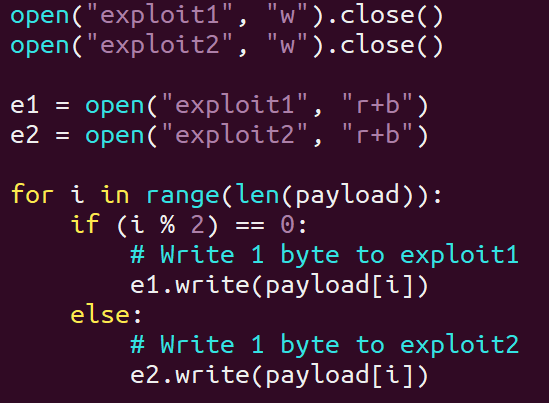
\includegraphics[scale=0.7]{./a2/buffer_overflow/alternate.PNG}\\

The next difficulty is, as mentioned in the tutorial pdf, overwriting of loop variables.\\\\
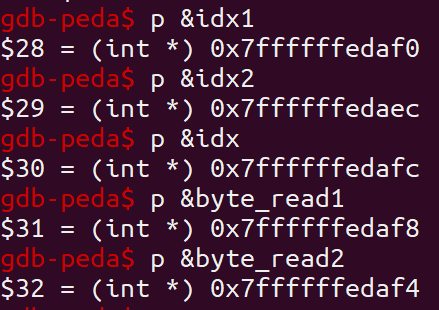
\includegraphics[scale=0.7]{./a2/buffer_overflow/extravariables.PNG}\\

The only relevant variables here are:
\begin{enumerate}
    \item \emph{byte\_read1}
    \item \emph{byte\_read2}
    \item \emph{idx}
\end{enumerate}
So to make sure that these values are consistent, our (full) payload will slot the values taken by these variables at runtime into the shellcode, like so:\\\\
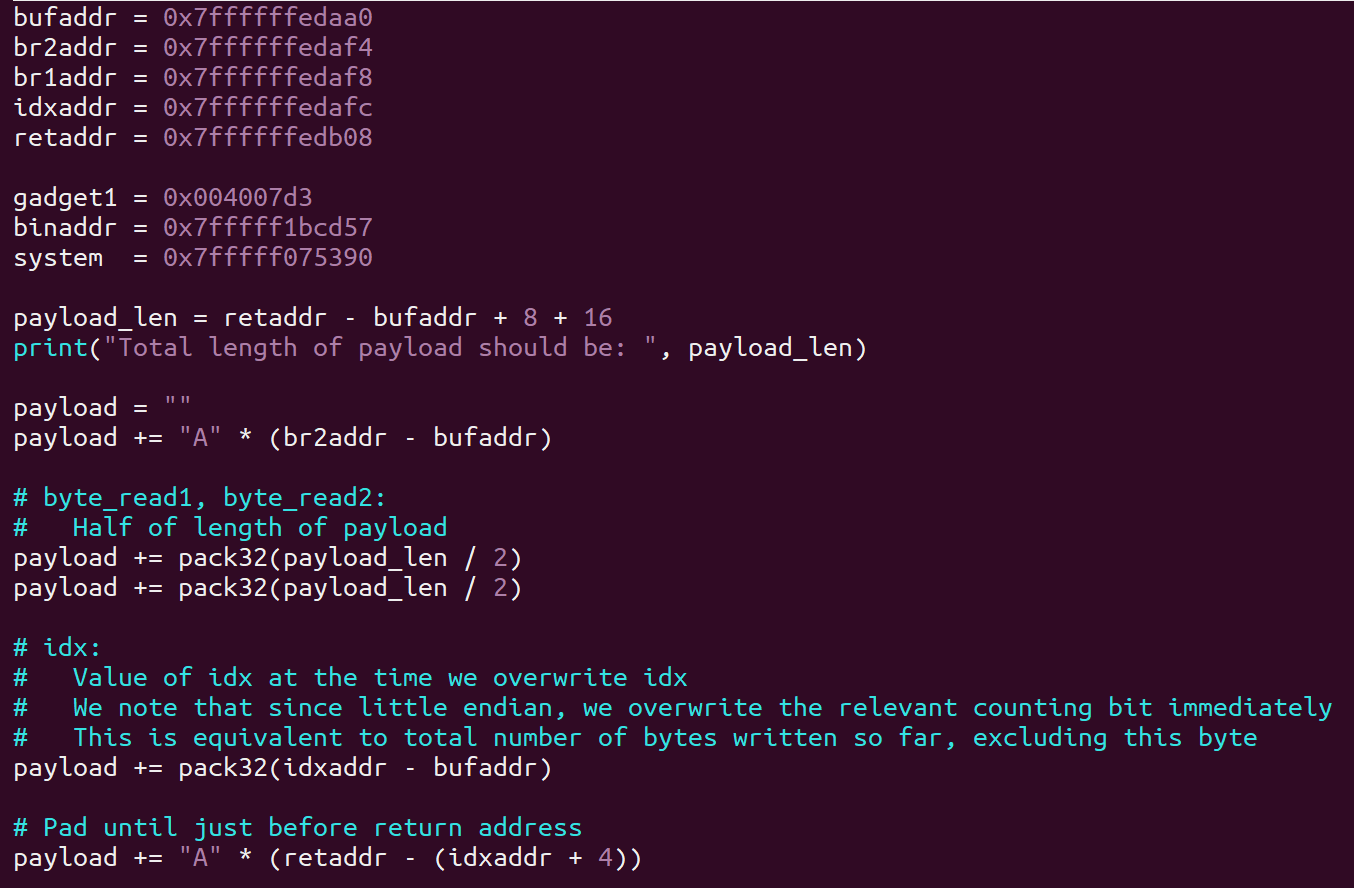
\includegraphics[scale=0.5]{./a2/buffer_overflow/extravariablesexploit.PNG}\\

The values of \emph{byte\_read1, byte\_read2} will be the half of the payload length (which corresponds to the length of files \emph{exploit1, exploit2}). The value of \emph{idx} trickier. In normal operation, it increments by 1 every time we (over)write a byte. Since we are working in a little endian system, the first byte we overwrite to \emph{idx} is the counting byte. So at that point in time, it is distance from the \emph{buf} address, excluding this first \emph{idx} byte.\\

To run the exploit, first run the program with any input. This will give us the buffer's starting address, with which we compute the rest of the local variable addresses using offsets from a locally compiled version of the program (refer to the above images), as shown below:\\\\
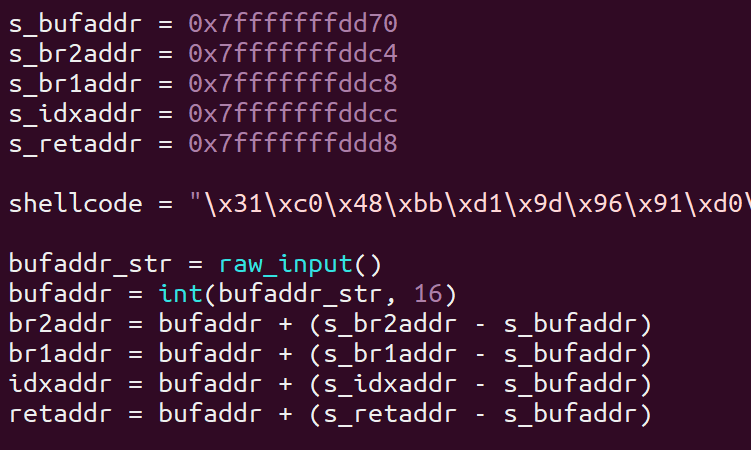
\includegraphics[scale=0.7]{./a2/buffer_overflow/offset.PNG}\\

Then give as input the hex address of the buffer starting location to the exploit script \emph{initexploit.py}, and it will generate the exploit files to be read. After that, run the program again. Below is a screenshot of it working.\\\\
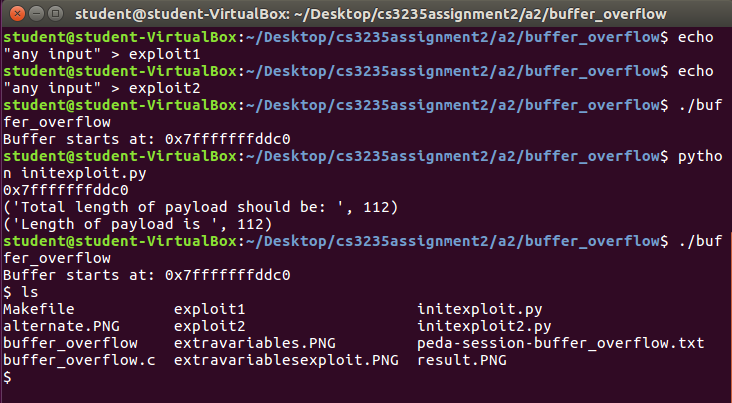
\includegraphics[scale=1]{./a2/buffer_overflow/result.PNG}

%======================================

\newpage
\section{Format String Attack}

The vulnerability is in the \emph{print(buf)} line, since we are using unsanitised user input as a format string. Overwriting the \emph{jackpot} variable is the same as Tutorial 2.\\

First, run the program with any input, which will output the \emph{jackpot} variable address.
Run the exploit-generating script \emph{initexploit.py} and feed the \emph{jackpot} variable address to the script.
This will generate the \emph{exploit} file.
Lastly, run the program and pipe in the \emph{exploit} file as input. See the 2 images below for the exact commands.\\\\

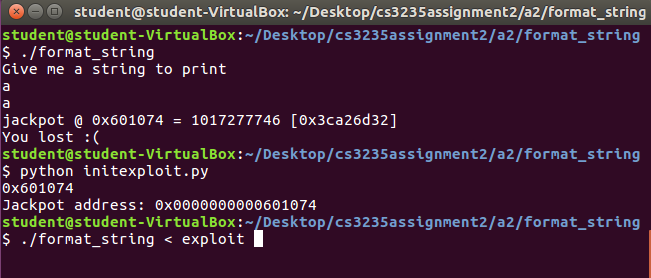
\includegraphics[scale=1]{./a2/format_string/result1.PNG}\\
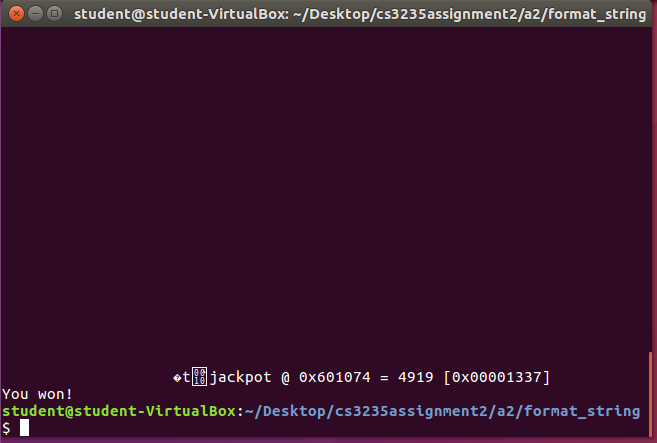
\includegraphics[scale=1]{./a2/format_string/result2.PNG}\\

The script to generate exploit file is as follows.\\\\

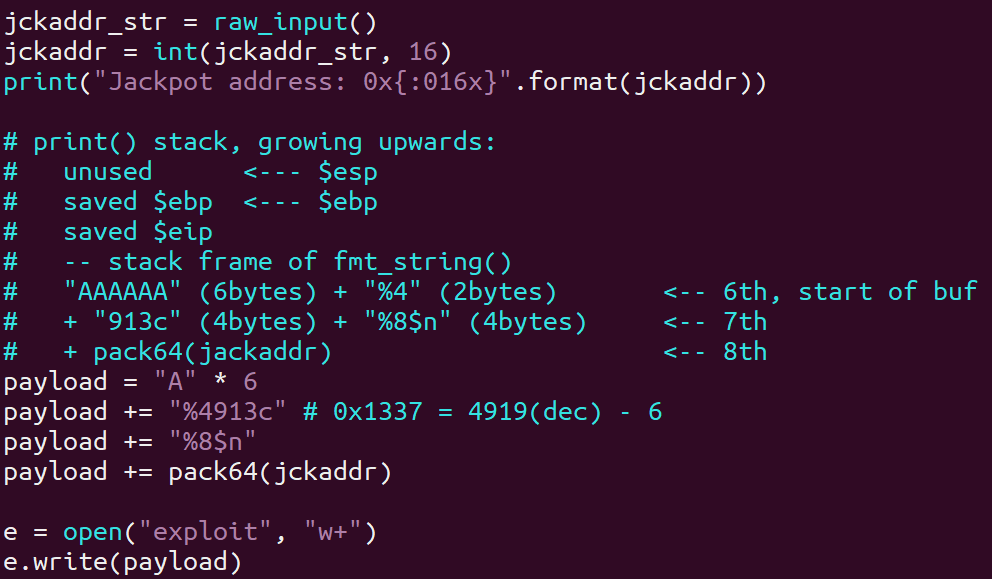
\includegraphics[scale=0.7]{./a2/format_string/script.PNG}\\

We first need to print $0x1337 = 4919$ characters, then place the format specifier \emph{\%8\$n} to write to the 8th positional argument with respect to the print stack frame.
As shown in the comments in the picture above, we place the address of the \emph{jackpot} exactly where the print function will retrieve the 8th positional argument from.
Last but not least, we align everything properly by padding the start with the character "A" and subtracting the number of "A"'s printed from the padded format specifer ($4919 - 6 = 4913$).


%======================================

\newpage
\section{Return-oriented Programming}

First, we can give as input a negative value which causes the check at line 12 to pass.
Coincidentally, casting signed variable (\emph{i}) to unsigned in line 21 causes negatively-valued signed values to be intepreted as (large) unsigned values.
Which means that \emph{read\_size} will likely take the value of \emph{fsize}, which is the size of the input \emph{exploit} file.
This could be more than the allocated buffer (\emph{buf}) size of $80$, which causes the overflow.\\

Now we have the overflow, we first need a way to extract stack addresses, and libc addresses. In particular, we need the stack address because stack addresses usually shift around (compared to GDB) due to extra environment variables.\\

In line 25, the program prints the \emph{buf}, which reads characters starting at the address of \emph{buf} until it encounters the NULL (\emph{0x00}) character. This is an information leak, allowing us to read off the stack data.\\\\

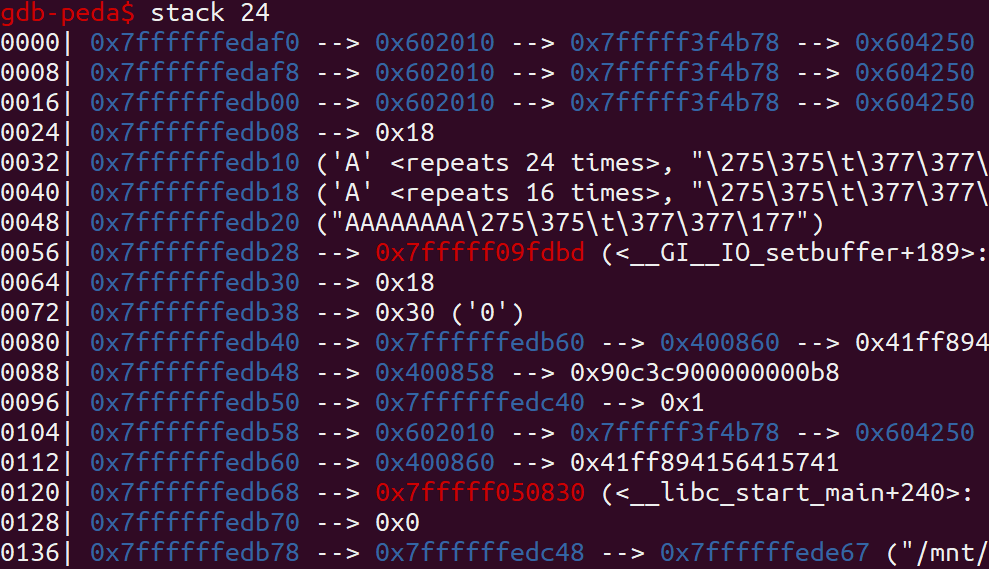
\includegraphics[scale=0.7]{./a2/rop/stack24.PNG}\\

The first piece of data we read is the saved EBP pointer, which references the stack.
This is located at address \emph{0x7ffffffedb40} as shown above.
The first script to run is \emph{initexploit1a.py}, which will generate an exploit file that fills up the stack until right before the address.\\\\

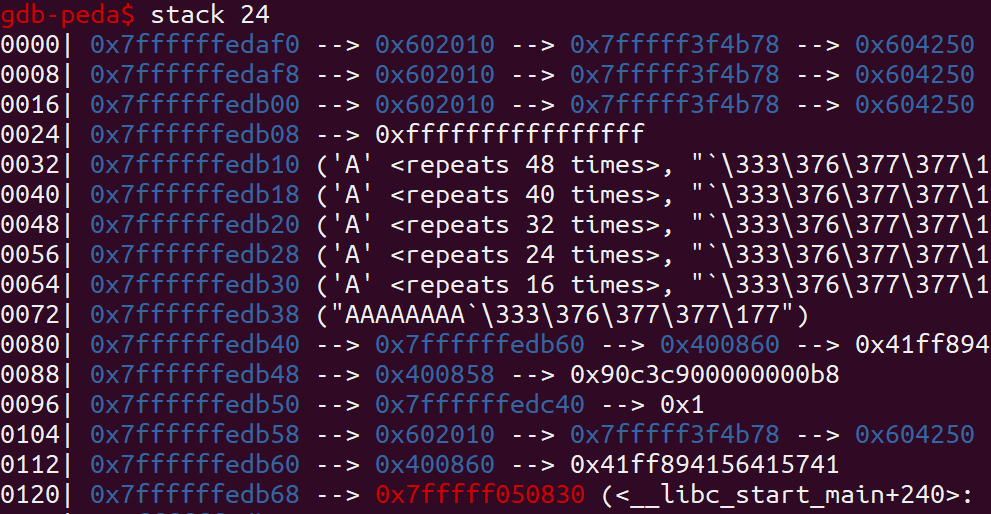
\includegraphics[scale=0.7]{./a2/rop/stack24_ebp.PNG}\\

Subsequently giving the program "-1" as input will print the full \emph{exploit} file to \emph{buf}.
Line 25 then prints starting from \emph{0x7ffffffedb10} (\emph{buf} address), until past the saved EBP address.
Dump the output to a file \emph{dump1}.
Examining the output using \emph{hexdump} reveals that the saved EBP is leaked (last few bytes).\\\\

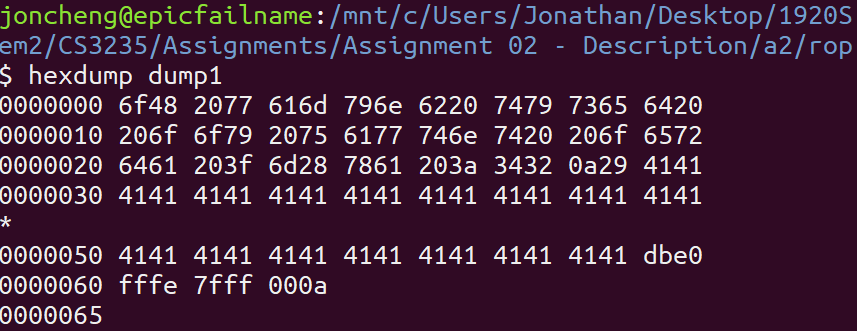
\includegraphics[scale=0.7]{./a2/rop/dump1.PNG}\\

Note that the full 8 bytes of the address is not leaked, since the last few \emph{0x00} bytes terminates the reading of \emph{puts}, and the last byte is \emph{0x0a} the newline character appended by \emph{puts}.\\

Then running \emph{initexploit1b.py} will extract the address from the dump, and return it.\\\\

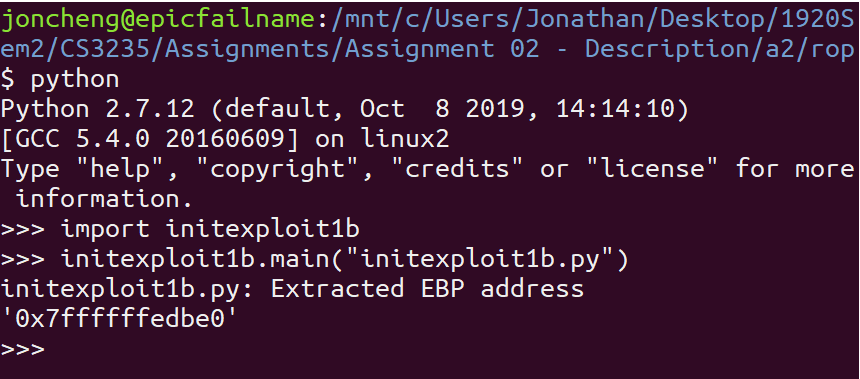
\includegraphics[scale=0.7]{./a2/rop/dump1_ext.PNG}\\

Now, the libc addresses. There are some assumptions not explicitly stated (or refuted) in the assignment pdf. I will list the scenarios which affect how to run the exploit.\\

\newpage
\subsection*{A: Victim machine arbitrary with GDB}
In this case, we have access to GDB, and the compiled binary.
Meaning we can extract all required addresses in libc from GDB.
Simply follow the tutorial and run the commands
\begin{enumerate}
    \item p open
    \item p read
    \item p write
    \item asm "pop rdi; ret" libc
    \item asm "pop rsi; ret" libc
    \item asm "pop rdx; ret" libc
\end{enumerate}
to find all the addresses and gadgets. Then simply hardcode the addresses into the \emph{initexploit\_vm.py} file like so:\\\\
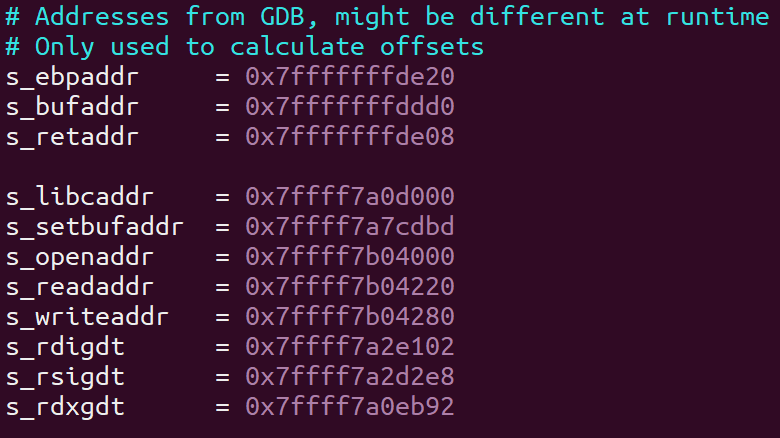
\includegraphics[scale=0.7]{./a2/rop/hclibc.PNG}\\

\newpage
\subsection*{B: Victim machine is the VM provided, no GDB}
We can still proceed by leaking a libc address from the stack.
Referring back to the untouched stack layout (first image of this task), we notice that address \emph{0x7ffffffedb28} holds a libc address.
We can perform the same information leak as the EBP one, with few modifications to get this address out.
The relevant script files are \emph{initexploit2a.py}, \emph{initexploit2b.py}.\\\\

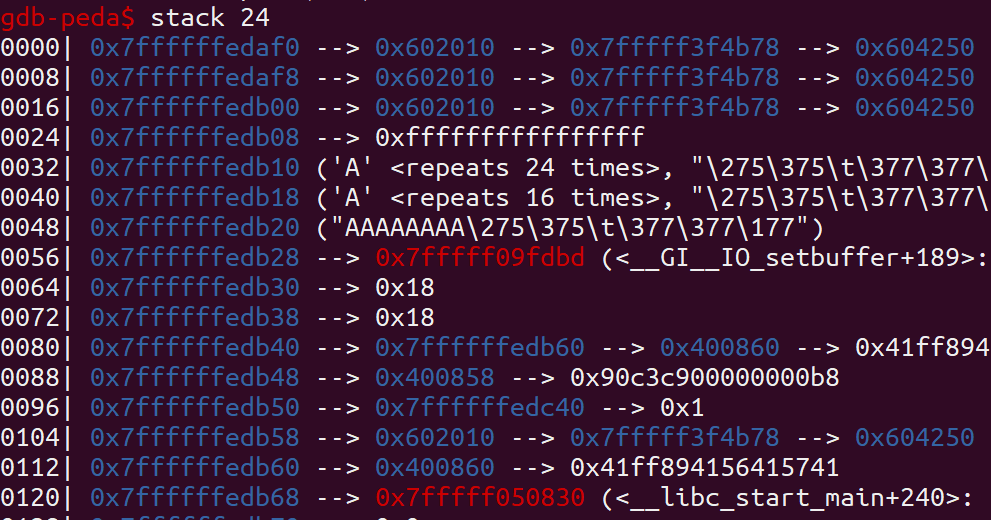
\includegraphics[scale=0.7]{./a2/rop/stack24_libc.PNG}\\
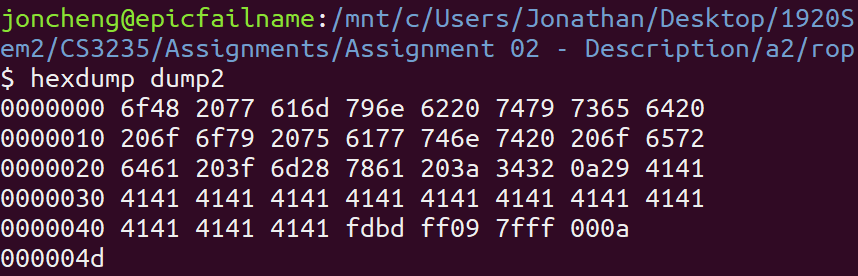
\includegraphics[scale=0.7]{./a2/rop/dump2.PNG}\\
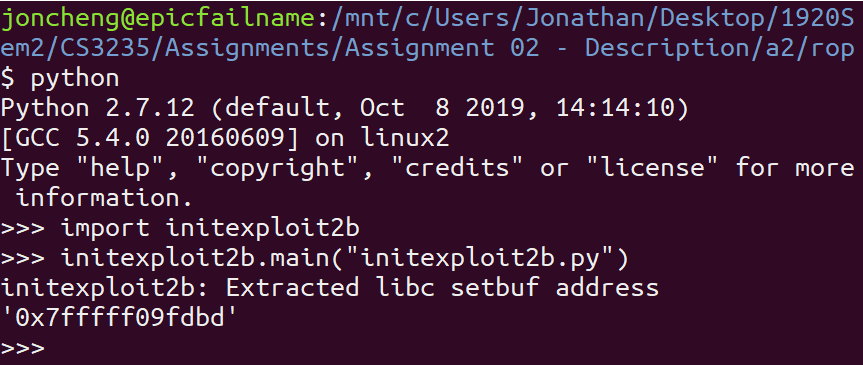
\includegraphics[scale=0.7]{./a2/rop/dump2_ext.PNG}\\

After which, we can compute the offsets for gadgets using addresses from GDB on a local machine. This is shown in the below image, where \emph{s\_*} variables are hardcoded addresses.\\\\

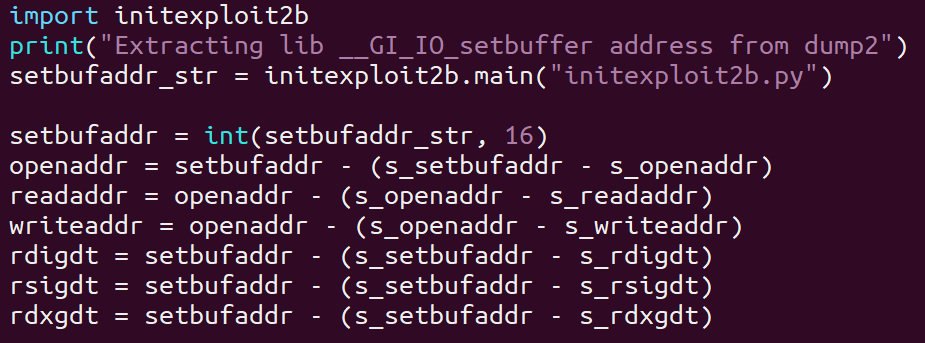
\includegraphics[scale=0.7]{./a2/rop/calclibc.PNG}\\

This is useful for scenario such as network attacks, where as an attacker we don't have access to the actual file binaries and only the output.
However, using this as a libc address may not be reliable (or even useful) since:
\begin{enumerate}
    \item We're using data leftover from a previous function call, not this \emph{rop} call. I tried to use the more reliable \emph{libc\_start} address, but this will mean I'll ovewrite the saved EBP/EIP addresses, causing the program to terminate without flushing the output buffer.
    \item We use the address to calculate offsets. Meaning it depends on the locally retrieved libc addresses (\emph{s\_*} variables) being accurate, which implies that the machine used to develop the exploit have the exact same libc binary as the victim machine, which is unlikely.
\end{enumerate}

\newpage
\subsection*{C: Victim machine is arbitrary, no GDB}
In this case, we will have to extract the libc addresses ourselves from the actual libc binaries.
In which case, we will need external tools to do so.
I'll list some relevant commands and links to do so:
\begin{enumerate}
    \item "LD\_TRACE\_LOADED\_OBJECTS=1 ./rop" can be used to get the base libc address
    \item "readelf -s /lib/x86\_64-linux-gnu/libc.so.6 $|$ grep open" to get the open (and read/write) address offset
    \item Use this tool \url{https://github.com/JonathanSalwan/ROPgadget} to search for gadgets' offsets, and add to libc base address
\end{enumerate}
Some images to show you it works:\\
libc base address:\\
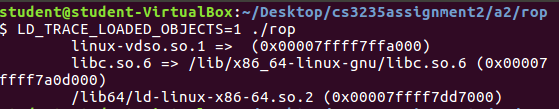
\includegraphics[scale=1]{./a2/rop/libcaddr.PNG}\\
open() offset:\\
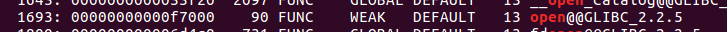
\includegraphics[scale=1]{./a2/rop/openoffset.PNG}\\
Then adding the two gives you:\\
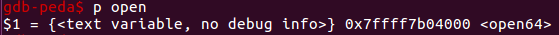
\includegraphics[scale=1]{./a2/rop/openaddr.PNG}

\newpage

In any case, once you get all the addresses, just need to craft the \emph{exploit} file.\\

We place the path of the file to be read at the start of \emph{buf}, and write to the stack right below where our payload ends (\emph{bufaddr} - len(\emph{exploit})).
The full payload looks like this:\\\\

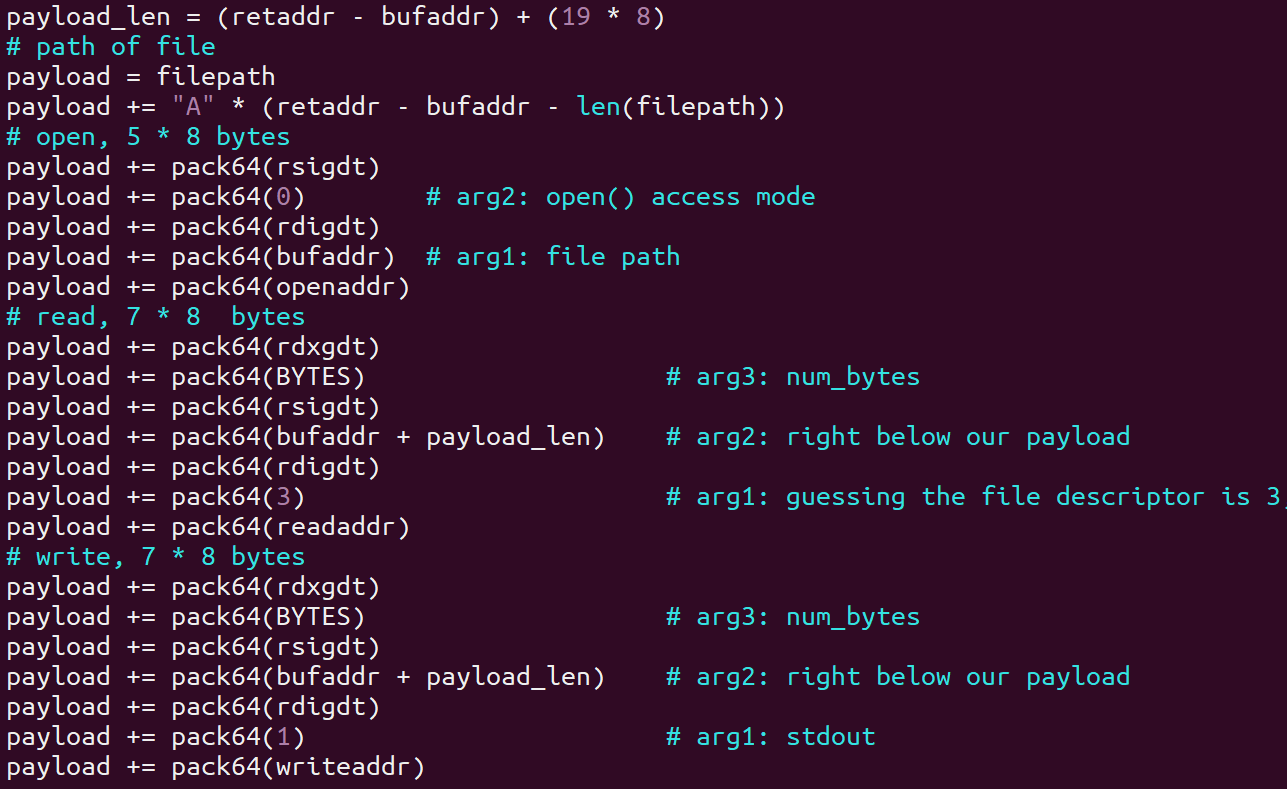
\includegraphics[scale=0.6]{./a2/rop/exploit.PNG}\\

There's not much to say, since this is really just copying the tutorial.
To run the full exploit, do the following in order:

\newpage
\textbf{Scenario A}:
\begin{enumerate}
    \item python initexploit1a.py; echo "-1" $|$ ./rop $>$ dump1
    \item python initexploit\_vm.py hclibc
    \item secret.txt
    \item 100
    \item echo -1 $|$ ./rop
\end{enumerate}
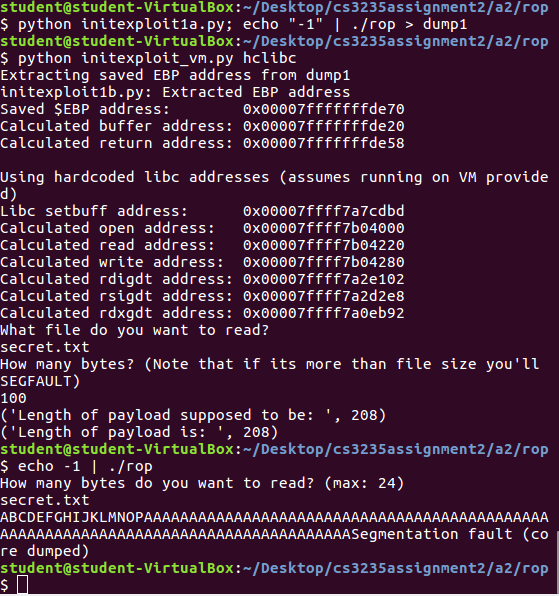
\includegraphics[scale=1]{./a2/rop/sceA.PNG}

\newpage
\textbf{Scenario B}:
\begin{enumerate}
    \item python initexploit1a.py; echo "-1" $|$ ./rop $>$ dump1
    \item python initexploit2a.py; echo "-1" $|$ ./rop $>$ dump2
    \item python initexploit\_vm.py
    \item secret.txt
    \item 100
    \item echo -1 $|$ ./rop
\end{enumerate}
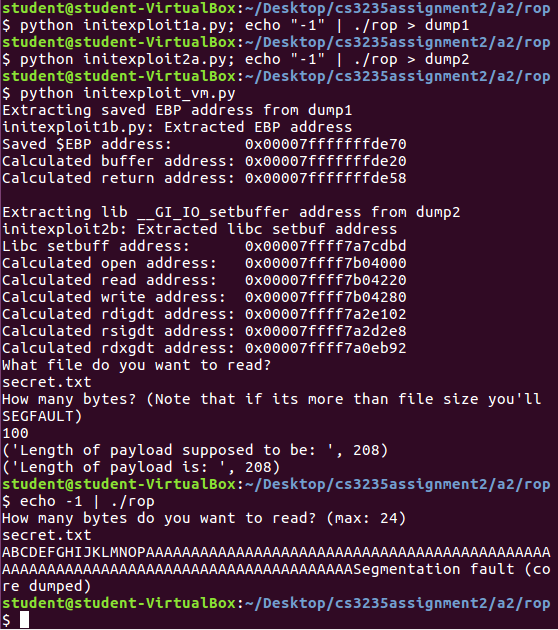
\includegraphics[scale=1]{./a2/rop/sceB.PNG}

\newpage
\textbf{Scenario C}:\\
You would first find the address, and replace the addresses of \emph{s\_*} variables in the \emph{initexploit\_vm.py} script. Then, run (same as A):
\begin{enumerate}
    \item python initexploit1a.py; echo "-1" $|$ ./rop $>$ dump1
    \item python initexploit\_vm.py hclibc
    \item secret.txt
    \item 100
    \item echo -1 $|$ ./rop
\end{enumerate}

\end{document}
